%!TEX root = ../../report.tex
\chapter{Experiments} % (fold)
\label{chap:experiments}
This chapter validates the ability of the ping pong ball catcher to determine the point of impact on the base plate, and move the arm to catch the ball once it bounces back.

\section{Catching the ball in time}
In order to validate that the calculations and movement of the servo is fast enough to catch a ping pong ball after it bounces back after a drop from $30\si{\centi\meter}$.
The ball is dropped over the centre of the plate, where the positioning system often calculates the impact point to be.
The arm moves in and catches the ball in time without trouble.
Based on this result it is concluded that the timing constraints on calculating where the arm should move to, and moving it there, are satisfied.

\section{Positioning}
In order to test whether the positioning system calculates the correct position, tests were conducted.
In each trial a ball is dropped above the same position on the base plate.
The target is 30 degrees from the $x$-axis and a distance of the arms length from the origo.
This target is marked with a red dot on figure \ref{fig:testRes30deg}.
As can be seen in the figure the positions of the impact points are calculated to be at very different places with each attempt. The reason to this error is differences in the timings as can be seen in figure \ref{fig:clockCycles30deg}.
\begin{figure}[htb]
	\centering
	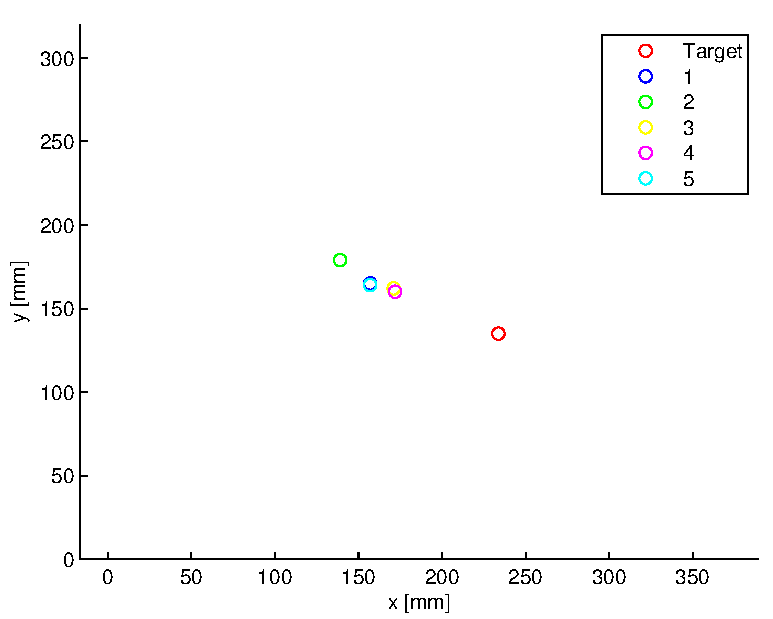
\includegraphics[width=.8\textwidth]{figures/testRes30deg.pdf}
	\caption{Estimated impact positions based as a result of dropping a ball on to the same target multiple times.}
	\label{fig:testRes30deg}
\end{figure}

In figure \ref{fig:timingPlot} the time difference between the four measurements on sensor $a$, $b$, $c$ and $d$ is indicated as blue, cyan and yellow respectively.
The values on $d$ cannot be seen since they are zero.
The measurements show a large variance for each trial. The sensor timings are not very consistent. In order to ensure that it is not the timing module that is causing these large errors it is validated.
%
\begin{figure}[htb]
	\centering
	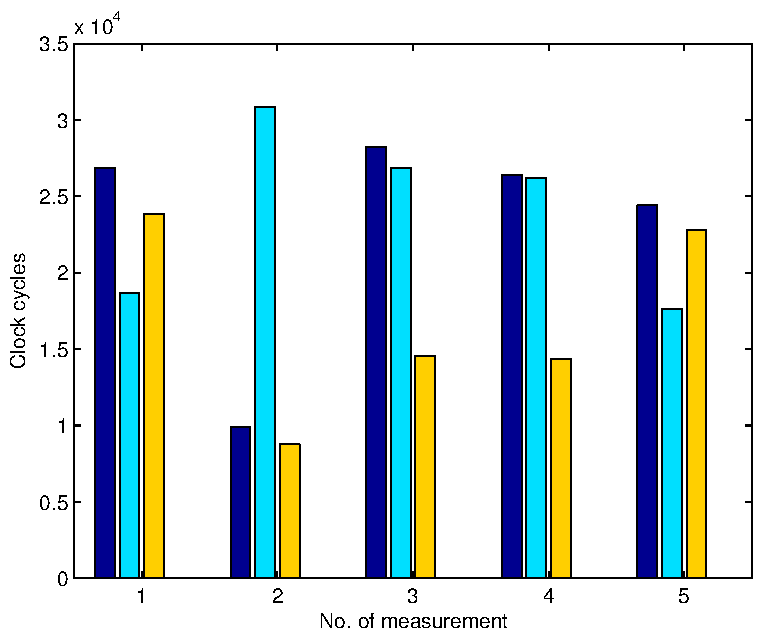
\includegraphics[width=.8\textwidth]{figures/clockCycles30deg.pdf}
	\caption{Estimated impact positions based as a result of dropping a ball on to the same target multiple times.}
	\label{fig:clockCycles30deg}
\end{figure}
%
\section{Validation of timing module}
To validate the timings the timing results from the timing VHDL component are compared with time difference calculated based on sampling the same sensor output on an oscilloscope. The sensor output can be seen on figure \ref{fig:timingPlot}. Timings to compare with are extracted by running through the sequence from the beginning until a value larger than the 2.4V are reach. The time at these points are stored for each sensor. The compare time values in table \ref{tbl:compareCycles} can be calculated by multiplying the time difference between each of the stored times and the smallest of them with the clock frequency the timing component counts with(50Mhz).

\begin{figure}[htb]
	\centering
	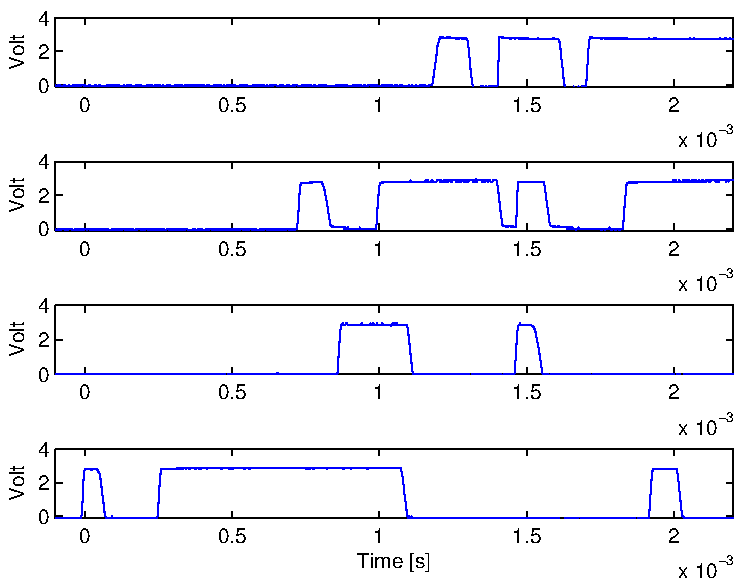
\includegraphics[width=.8\textwidth]{figures/timingPlot.pdf}
	\caption{Estimated impact positions based as a result of dropping a ball on to the same target multiple times.}
	\label{fig:timingPlot}
\end{figure}
%
\begin{table}[h]
	\begin{tabular}{|l|l|l|l|l|}
		\hline
		 & ta & tb & tc & td \\
		 \hline
		Difference in cycles from timing module & 36655 & 59827 & 43481 & 0 \\
		 \hline
		Difference in cycles from oscilloscope & 36600 &  60000 &  43400 & 0 \\
		\hline
	\end{tabular}
	\caption{Comparison of clock cycles from timing module and calculated from oscilloscope data.}
	\label{tbl:compareCycles}
\end{table}
%
As can be seen from table \ref{tbl:compareCycles} the compare values are roughly the same. Hence it is concluded that the timing is correct, so the fault must be before the FPGA in the system.
% chapter experiments (end)